%
% File acl2017.tex
%
%% Based on the style files for ACL-2015, with some improvements
%%  taken from the NAACL-2016 style
%% Based on the style files for ACL-2014, which were, in turn,
%% based on ACL-2013, ACL-2012, ACL-2011, ACL-2010, ACL-IJCNLP-2009,
%% EACL-2009, IJCNLP-2008...
%% Based on the style files for EACL 2006 by 
%%e.agirre@ehu.es or Sergi.Balari@uab.es
%% and that of ACL 08 by Joakim Nivre and Noah Smith

\documentclass[11pt,a4paper]{article}
\usepackage[hyperref]{acl2017}
\usepackage{times}
\usepackage{latexsym}
\usepackage{amsmath}
\usepackage{amsfonts}
\usepackage{algorithm}
\usepackage{algpseudocode}
\usepackage{graphicx}
\usepackage{footnote}
\usepackage{footmisc}
\usepackage{footnotebackref}
\newcommand*\Let[2]{\State #1 $\gets$ #2}  
\usepackage{url}


%\aclfinalcopy % Uncomment this line for the final submission
%\def\aclpaperid{***} %  Enter the acl Paper ID here

%\setlength\titlebox{5cm}
% You can expand the titlebox if you need extra space
% to show all the authors. Please do not make the titlebox
% smaller than 5cm (the original size); we will check this
% in the camera-ready version and ask you to change it back.

\newcommand\BibTeX{B{\sc ib}\TeX}

\title{NLP2 project 1}

\author{Tim van Elsloo \\
 10590315\\\And
  Fije van Overeem \\
  10373535 \\\And 
  Daan van Stigt \\
  10255141    }

\date{}

%%%
% I think as a rule of thumb we should explain each model and 'extension' (VI and ELBO) using:
% 
% a) natural language:
%    - what are we doing
%    - why is it necessary to do it this way (e.g. why elbo?)
%    - what are the assumptions we are making
%    - what is the main difference with all other things we are discussing
%        i.  EM vs VI
%        ii. Log-likelihood vs ELBO
% b) the maths involved
% c) an efficient algorithm in pseudocode
%%%



\begin{document}
\maketitle
\begin{abstract}
This paper reports on a series of experiments conducted with the IBM models 1 and 2. For both models the parameters are estimated from a parallel corpus. These parameters are used to predict alignments on a test set. The alignments are evaluated against gold standard alignments and the alignment error rate (AER) is recorded. We experiment with two different methods of parameter estimation for IBM1, and three different methods of initialising the parameters of IBM2.
\end{abstract}

\section{Introduction}

The IBM models \cite{brown1993} lay the groundwork for much current research in statistical machine translation. Although the models were originally designed for the task of full translation, they are nowadays used mostly for the prediction of word alignments in translated sentence pairs. IBM1 and IBM2 are statistical models. 

% The produced word alignments can then for example be used for the for translation models between a source language and a target language.
In this paper we will report on the results of a series of experiments performed with the IBM1 and IBM2 models. For IBM1 we experiment with two different methods for parameter-estimation: expectation maximisation (EM); and variational inference, for a Bayesian formulation of the model. For IBM2 we experiment with three different methods of initialising the translation parameters: uniformly, like in IBM1; randomly; and initialisation using pre-trained parameters obtained from a trained IBM1 model. Because of the non-convexity of IBM2, each of these initialisations yield different results.



%%% What's this? Hier databeschrijving, deze punten vielen me op bij lezen van papers dat we dat misschien kunnen noemen.
% \section*{Data}
% \begin{itemize}
%     \item Following Collins, we call our data partially observed, because we don't know the alignments for the training examples.
%     \item Amount of French and English sentences.
% \end{itemize}

% \section*{Assumptions for all IBM models}
% % random sticky note: the likelihood function of the models usually has multiple optima
% \begin{itemize}
%     \item Independence between sentence pairs is assumed
% \end{itemize}
% \section*{Experiments}
% \subsection*{IBM1}
% \subsubsection*{Underlying assumptions of the model}
% \begin{itemize}
%     \item 
% \end{itemize}
% \subsection*{IBM2}
% \begin{itemize}
%     \item The distribution
% of the random variable $A_i$ depends only on the values for the random variables
% $L$ and $M$ (it is independent of the English words $E_1$ . . . $E_l$, and of the other alignment
% variables) (p.8 Collins).
%     \item 
% \end{itemize}
%%%

\section{Models} 

The IBM models 1 and 2 are both alignment models: they predict how each word in a sentence aligns to a word in the translated sentence. The two models are identical and differ only in their alignment assumptions. IBM1 assumes that alignments between any two sentences positions are equally likely; IBM2 additionally trains these alignments. We discuss how the two models are defined below, starting with IBM1.

\subsection{IBM 1}

% The simplest model that we have implemented is IBM Model 1
% , with its parameters estimated standard with EM. 
% In IBM Model 1, our goal is to estimate the probability of a French word given an English word $t(f | e)$, where our motivation is to be able to translate a whole corpus. If we find alignment links that give us the highest probability for each $t(f|e)$, we could use these alignment links to translate a whole corpus.
The simplest model that we have implemented is IBM Model 1. Following \citet{schulz}'s tutorial, we start by defining a joint probability over a parallel corpus $C$ consisting of translated sentence pairs $(e_1^{l}, f_1^{m})$ as follows:
\begin{align*}
    P(C)=\prod^{|C|}_{s=1}P(e_1^{s_l}, f_1^{s_m}).
\end{align*}
This assumes all sentence pairs to be independent\footnote{Using the multiplication rule for independent events}. This is the first simplifying assumption used with IBM models that derogates natural languages, whereas sentences are in fact not independent of one another.
This assumption is simplifying in the sense that we from now on only have to consider individual sentence pairs, as statements about them are easily extended to a whole corpus because of the independence assumption. 
We are interested in modelling the probability $P(e_1^{s_l}, f_1^{s_m})$. Using the chain rule of probability this can be decomposed:
\begin{align*}
    P(e_1^{l}, f_1^{m})=P(e_1^l) P(f_1^m|e_1^l)
\end{align*}
in which we can identify a language model $P(e_1^l)$ and the translation model $P(f_1^m|e_1^l)$. The the language model models the probability of the English sentence, and for this any language model could be used. The translation model is the part that IBM1 and IBM2 are designed to model. This is the probability of a French sentence, given an English sentence. To model this probability, IBM1 introduces an alignment variable $a_j$ for each word $f_j$ in the French sentence. For each $j\in \{1,\dots,m\}$ the alignment variable $a_j$ can take any value in $\{0,....,l\}$ indicating which English word $e_{a_j}$ the French word $f_j$ is aligned with. Thus this alignment variable will align each French word with one word in the English sentence.

The probability $P(f_1^m, a_1^m|e_1^l)$---which includes the alignment variables---is then modelled as:
\begin{align*}
    P(f_1^m, a_1^m|e_0^l) &= \prod^m_{j=1}P(a_j|m, l) P(f_j | e_{a_j}) \\
        &= \prod^m_{j=1}\frac{1}{l+1} P(f_j | e_{a_j}) \\
        &= \frac{1}{(l+1)^m} \prod^m_{j=1} P(f_j | e_{a_j})
\end{align*}
where $P(a_j|m, l) = \frac{1}{l+1}$ expresses the fact that in IBM1 the probability of French word $j$ aligning to English word $a_j$ given sentence lengths $m$ and $l$ is assumed to be uniform. Marginalizing the $a_j$ gives us then that
\begin{align*}
    P(f_1^m |e_0^l) &= \prod^m_{j=1} \frac{1}{(l+1)^m} \sum_{a_j=0}^l  \dot P(f_j | e_{a_j}).
\end{align*}
Hence the full likelihood of the corpus $C$ under the model is given by
\begin{align}
    \prod_{(f_1^m,e_0^l)\in C}\prod_{j=1}^m  \frac{1}{(l+1)^m}\sum_{a_j=0}^l P(f_j | e_{a_j}).
\end{align}

The training task is to estimate the parameters $P(f_j | e_i)$ from the training corpus. We have implemented two methods for this: Expectation Maximisation (EM); and Variational Inference (VI) for the Bayesian version of the above model that will be discussed below.

% (sec. \ref{sec:em1}) and Variational Inference (sec. \ref{sec:vi1}).



% This probability is denoted by the following
% \begin{align*}
%     P(f_1^m|e_1^l)=\frac{1}{(l+1)^m}\prod^m_{j=1}\sum^l_{i=0}t(f | e)
% \end{align*}

% \subsubsection{Problems with IBM1-EM}
% The IBM1 model is problematic in a couple of ways. We summarize these problems following \citet{moore} who investigated on improvements on IBM1:
% \begin{itemize}
%     \item The model assumes all words in the target sentence can only be generated by one word in the source sentence. This even though, in natural languages, multiple words sometimes translate into one word.
%     \item Sentences are treated as a bag-of-words, even though the place of a word in a sentence tells a lot about its translation.
%     \item Whether a particular source word is
% selected to generate the target word for a given
% position is independent of which or how many
% other target words the same source word is selected
% to generate.
% \end{itemize}


\subsubsection{Expectation Maximisation}

\label{sec:em1}

The EM algorithm is a method to find the maximum likelihood estimates of parameters in a statistical model with latent variables. The EM-algorithm performs two steps alternatingly: in the E-step it gathers expected counts under the approximate distribution obtained in the previous step; in the M-step it updates the parameters by choosing the parameters that maximizes the log-likelihood of the counts gathered in the E-step.

In the case of IBM1 the E-step consists of collecting expected counts for the events 
\begin{align*}
    c(e,f) &= \mathbb{E}[\#(e \to f)] \\
        % &= \sum_{(f_1^m,e_0^l)\in C}\sum_{j=1}^m \sum_{a_j=0}^l P(a_j = i | f_j, e_0^l).\\
    c(e) &= \sum_f c(e,f)
\end{align*}
and in the M-step $P(f | e)$ is re-estimated as:
\begin{align*}
    P(f | e) = \frac{c(e,f)}{c(e)}
\end{align*}
Hence, the expectation step consists of iterating through all sentence pairs in the dataset and counting the co-occurrence of words in for pair using expected counts. So we count $P(f | e)$, the number of times a French word $f$ occurs in a translation of a sentence that contains English word $e$. 

% The subsequent maximization step is shown in eq. \ref{eq:em1-max}.

% \begin{align}
%     P(f_j | e_i) = \frac{c(f | e)}{\sum_f c(f | e)} \label{eq:em1-max}
% \end{align}

% \begin{algorithm}[H]
%     \begin{algorithmic}[1]
%         \Statex Count normalizers:
%         \For{E, F sentences}
%             \For{$f \in F$}
%                 \Let{$N_f$}{$\sum_{e \in E} t(f | e)$}
%             \EndFor
%         \EndFor
        
%         \Statex
%         \Statex Count probabilities:
%         \For{E, F sentences}
%             \For{$f \in F$}
%                 \For{$e \in E$}
%                     \Let{$\delta$}{$\frac{t(f | e)}{N_f}$}
%                     \Let{$c(f, e)$}{$c(f, e) + \delta$}
%                     \Let{$c(e)$}{$c(e) + \delta$}
%                 \EndFor
%             \EndFor
%         \EndFor
        
%         \Statex
%         \Statex Update translation probabilities:
%         \For{$e \in \mathcal{E}, f \in \mathcal{F}$}
%             \Let{$t(f | e)$}{$\frac{c(f, e)}{c(e)}$}
%         \EndFor
%     \end{algorithmic}
%     \caption{Iterative update for EM of IBM 1}
%     \label{algo:ibm1}
% \end{algorithm}

\subsubsection{Variational Inference}

\label{sec:vi1}

% Here Moore's paper can explain why and when EM does not suffice.
Our second experiment for IBM Model 1 is to extend it into a Bayesian model. We now assume a prior we now assume a $\text{Dir}(\alpha)$ prior on our translation parameters. The intractable posterior that we obtain this way is approximated using the method of variational inference:

\begin{align*}
    \phi_j &= \frac{
        \exp \left( \Psi \left( \lambda_{f_j | e_{a_j}} \right) - \Psi \left( \sum_f \lambda_{f | e_{a_j}} \right) \right)
    }{
        \sum_{i = 0}^m \exp \left( \Psi \left( \lambda_{f_j | e_i} \right) - \Psi \left( \sum_f \lambda_{f | e_i} \right) \right)
    } \\
    \lambda_{f | e} &= \alpha_f + \sum_{(e_0^m, f_1^n)} \sum_{j = 1}^n \mathbb{E}_{Q(A_j | \phi_j)}[\#(e \to f | A_j)]
\end{align*}

% \begin{algorithm}[H]
%     \caption{Iterative update algorithm for variational inference of IBM 1}
%     \begin{algorithmic}[1]
%         \Let{$\lambda_{f | e}$}{$\alpha_f$} \Comment{Initialize translation probabilities}
%         \For{blabla} % xxx
        
%         \EndFor
%     \end{algorithmic}
% \end{algorithm}

After conducting a brief pilot study, we have selected a symmetric prior $\alpha = 10^{-1}$.

\subsubsection{ELBO}

% MLE is a sort of KL-divergence minimalization. But we can't minimize it directly, so we approximate with ELBO.

For the Bayesian model, we use the evidence lower bound (ELBO) instead of the likelihood. We can rephrase our likelihood maximization problem into a KL-divergence minimalization problem. However, we can't minimize the KL-divergence directly. The ELBO provides a lower bound of the evidence and maximising the ELBO minimizes the KL-divergence, which in turn maximizes the likelihood function.

\begin{align*}
    \sum_{j = 1}^m \mathbb{E}_q [ \log P(a_j | m) P(f_j | e_{a_j}, \theta) - \log Q(a_j | \phi_j)] \\
    + \sum_e \mathbb{E}_q [ \log p(\theta_e | \alpha) - \log q(\theta_e | \lambda_e)]
\end{align*}

We have computed the ELBO using the equations published in \citet{schulz2}.

\subsection{IBM 2}

IBM2 revisits the independence assumption on the alignment probabilities $P(a_j|j, m, l)$ made by IBM1. In IBM2, these probabilities are additionally estimated from the data. This means that for IBM2 the joint probability of a French sentence $f_1^m$ and alignments $a_1^m$ given an English sentence 
$e_1^l$ is given by

\begin{align*}
    P(f_1^m, a_1^m|e_1^l) &= \prod^m_{j=1}P(a_j|j, m, l) P(f_j | e_{a_j}). \\
\end{align*}
Note that with $P(a_j|j, m, l)$ we have now introduced a probability distribution over English sentence positions $a_j \in \{0,\dots,l\}$ for \textit{each triple} $(j,m,l)$ of French word position $j$, French sentence length $m$, and English sentence length $l$. 

This means that for IBM2 the complete likelihood of the corpus is given by:
\begin{align}
    \prod_{(f_1^m,e_0^l)\in C}\prod_{j=1}^m  \sum_{a_j=0}^lP(a_j|j, m, l)  P(f_j | e_{a_j}).
\end{align}


% Appropriately initialising parameters for IBM Model 2 is difficult and it converges to a different local optimum depending on those parameters. Therefore, instead of initialising randomly, we have also used IBM Model 1 to initialise the parameters for IBM Model 2.

\subsubsection{Jump parametrisation}

The above parametrisation of the alignment probability $P(a_j=i|j, m, l)$ is very costly. In order to make estimation of this probability more efficient a different parametrisation based on a so-called jump-function is used, following \cite{Vogel:1996}. First, we define a jump-function
\begin{align*}
    \delta(i,j,m,l) = i - \left \lfloor{l\frac{j}{m}}\right \rfloor 
\end{align*}
for each $i,j,m,l$, where $i\in\{0,\dots,l\}$ and $j \in \{1,\dots,m\}$. The function $\delta$ measures how much of a jump is made when a word in the $j$th position of a sentence of length $m$ is aligned to a word in the $i$th position in sentence of length $l$, scaled to the respective sentence lengths.

The alignment distribution is then defined as
\begin{align*}
    P(a_j=i|j, m, l) = \text{Cat}(\Delta |\theta_{\delta(i,j,l,m)})
\end{align*}
where: $\Delta = (-k,\dots,0,\dots,k)$ is the range of possible jumps that an alignment can make, for some maximal value for an alignment-jump $k$; $\theta = (\theta_{-k},\dots,\theta_{k})$ is the parameter-vector that holds the probabilities for each jump-event $-k$ to $k$; and $\delta(i,j,l,m)$ is used to determine the index in this vector and hence the probability of jumping a distance $\delta(i,j,l,m)$.

\subsubsection{Parameter estimation}

Parameter estimation in IBM2 is performed only with EM. The estimation of is identical to IBM1 with the exception that the expected counts in the E-step are now gathered with respect to the the likelihood in formula (2), which includes the jump probabilities. 

\section{Prediction of alignments}
Given their estimated probabilities, IBM1 and IBM2 can predict alignments. For this we need the posterior probability of an alignment link, given by
\begin{align*}
    P(a_j = i | f_j, e_0^l, m) &= \frac{P(i|j,m,l)P(f_j|e_i)}{\sum_{i=0}^l P(i|j,m,l)P(f_j|e_i)} \\
    &= \frac{P(f_j|e_i)}{\sum_{i=0}^l P(f_j|e_i)} \text{   for IBM1.}
\end{align*}
When aligning two sentences we pick the alignment $a_1^m$ with the highest posterior probability. Since alignments are assumed to be independent we align each French word independently: we align French word $f_j$ to the English word $e_{a_j}$ for which $P(a_j = i | f_j, e_0^l, m)$ is maximal. This gives us our predicted sentence alignment.


\section{Experiments}

In order to compare IBM1-EM, IBM1-VI and IBM2 we propose an experimental setup that compares the alignment error rates (AERs) of each model that we have presented in this paper.

Our training data consists of 231k sentences selected from Canadian parliamentary proceedings\footnote{The Hansard French/English corpus. Source https://catalog.ldc.upenn.edu/LDC95T20}. These sentences were written in either English or French, and then translated to the alternative language by hand.

We run each model on all training data for 14 iterations. At each iteration, we use the model to make predictions on the validation data and compute the AER. For each model, we select the parameters of its best iteration with respect to the log-likelihood of the training data and the AER of the validation data.

In addition, we have repeated the training of IBM2-EM with random initialisation three times, in order to determine the magnitude of its significance on the final AER.

Experiments performed on our IBM1-VI model are constrained to 10k sentences due to exhaustion of resources above that level. We will therefore only compare the performance of IBM1-EM and IBM1-VI on 10k sentences both.

The coded implementation can be found on https://github.com/elslooo/nlp2.

\subsection{Results}
In table \ref{table:results-1} we demonstrate the AER of the best models for IBM1 on the test set for IBM1-EM and IBM1-VI.
In table \ref{table:results-2} we see the best AER scores for the IBM2 model with the five different initial parameter settings. The AER of the IBM1-initialised model is the lowest and thus has produced the best alignment links for IBM2.
In figure \ref{fig:jump-plot} it is demonstrated how the jump distribution gets more and more skewed around 0 after each iteration.
\begin{savenotes}
\begin{table}
\begin{tabular}{ |p{2cm}||p{2cm}||p{2cm}| }

 \hline
    & AER & Selected by\\
 \hline
 EM    &  0.2867 & likelihood \\
 VI   &  0.4114\protect\footnote{Trained on 10k sentences instead of 231k.}   & likelihood \\
 \hline
\end{tabular}
\caption{Results of best models for IBM1 on test set. How models were selected based on validation set is indicated.}
\label{table:results-1}
\end{table}
\end{savenotes}

\begin{table}
\begin{tabular}{ |p{2cm}||p{2cm}||p{2cm}| }
 \hline
    & AER & Selected by \\
 \hline
 uniform    &  0.2643  &    likelihood \\
 random 1   & 0.2646   &   likelihood \\
 random 2   & 0.2741   &   likelihood \\
 random 3   & 0.2640   &    likelihood \\
 IBM1 init      & 0.2637  &    likelihood \\
 \hline
\end{tabular}
\caption{Best results for IBM2 on test set. How models were selected based on validation set is indicated.}
\label{table:results-2}
\end{table}


\section{Conclusion}

We have implemented IBM Model 1 and 2 with Expectation Maximisation and Variational Inference. We have seen that IBM1-EM already performs surprisingly well with respect to its AER. In our experiments, IBM1-VI is outperformed by IBM1-EM, however we acknowledge that this is inconclusive due to the lack of training because of constraint resources. IBM Model 2 expands on 1 in the sense that it no longer assumes that the distribution over alignments is uniform, and instead estimates this probability distribution as well. 
It is interesting to see that the IBM2-runs with random initialisation differ a lot in the beginning but at the end, around epoch 8, converge to the same AER. We could conclude that the initial state for IBM2 does not influence the quality of the alignment after a certain amount of epochs but statistical testing is necessary to ascertain this. 

\bibliography{acl2017}
\bibliographystyle{acl_natbib}


% \section*{Figures}

\begin{figure}
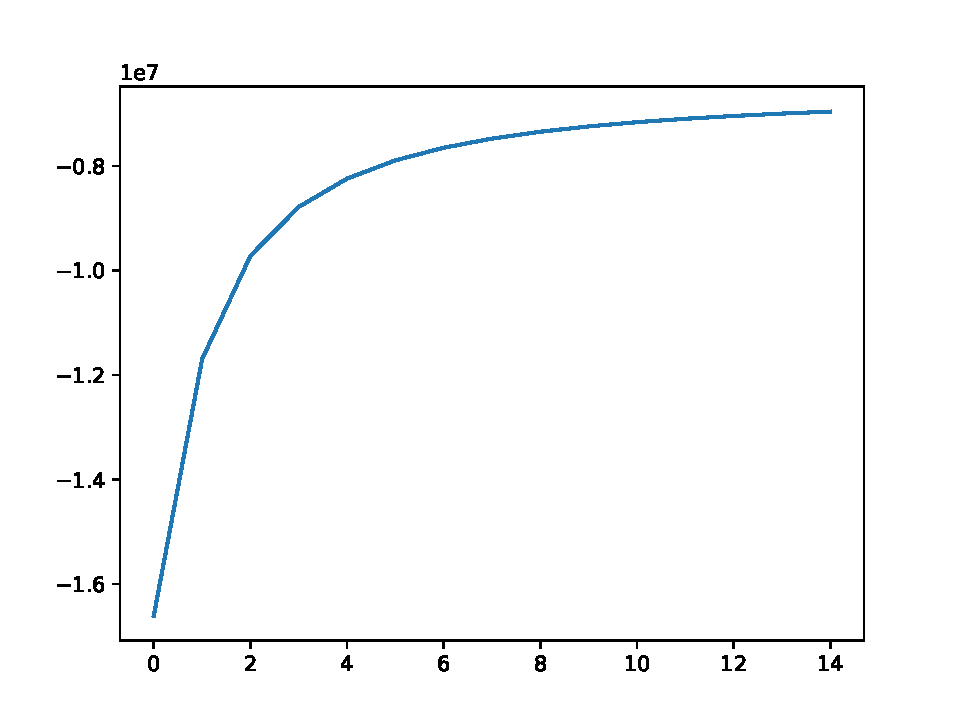
\includegraphics[width=\linewidth]{images/log-likelihood.pdf}
\caption{Log-likelihood of the training set for IBM1-EM plotted per epoch}
\label{fig:ll-1}
\end{figure}

\begin{figure}
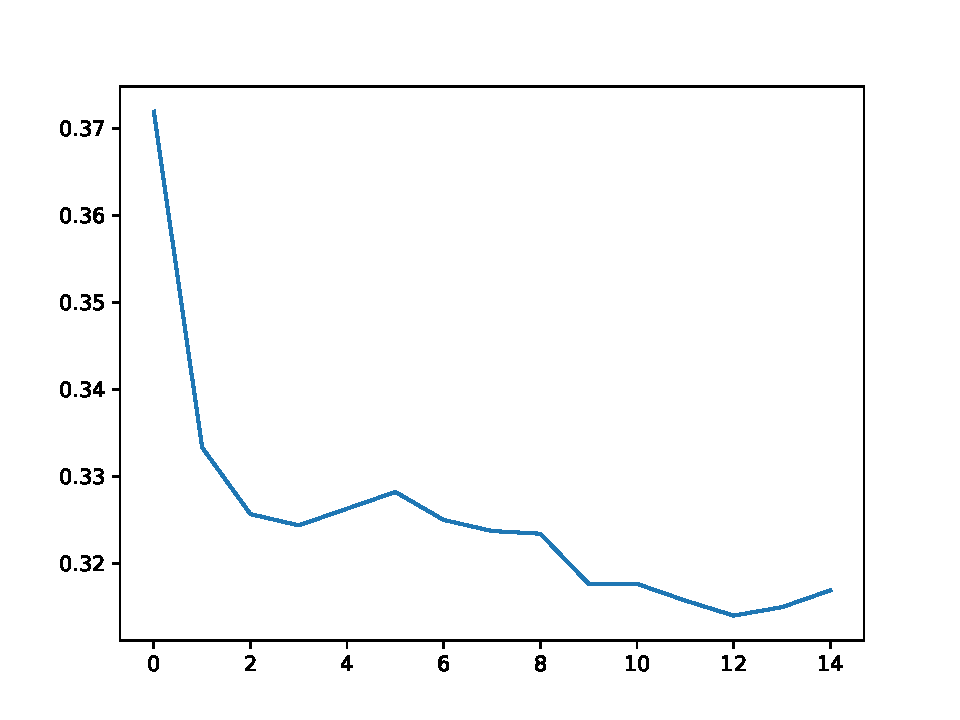
\includegraphics[width=\linewidth]{images/AER-plot.pdf}
\caption{AER on the development set for IBM1-EM plotted per epoch}
\label{fig:AER-1}
\end{figure}

\begin{figure}
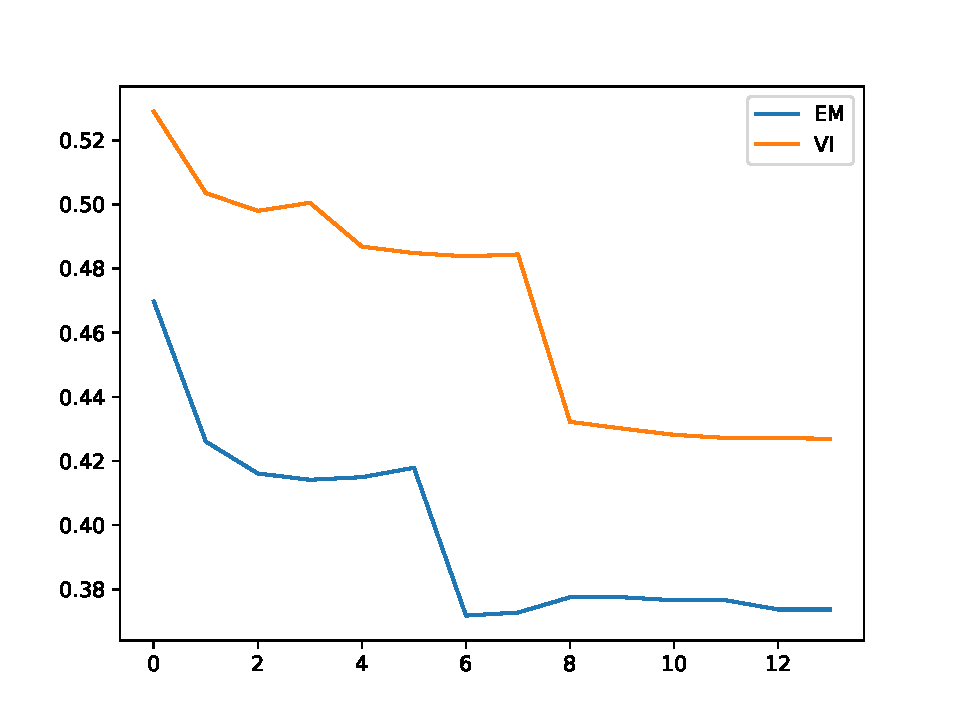
\includegraphics[width=\linewidth]{images/VI-AERs-together.pdf}
\caption{AER on a 10k subset of the development set for IBM1-VI and IBM-EM plotted per epoch}
\label{fig:VI-AER}
\end{figure}

\begin{figure}
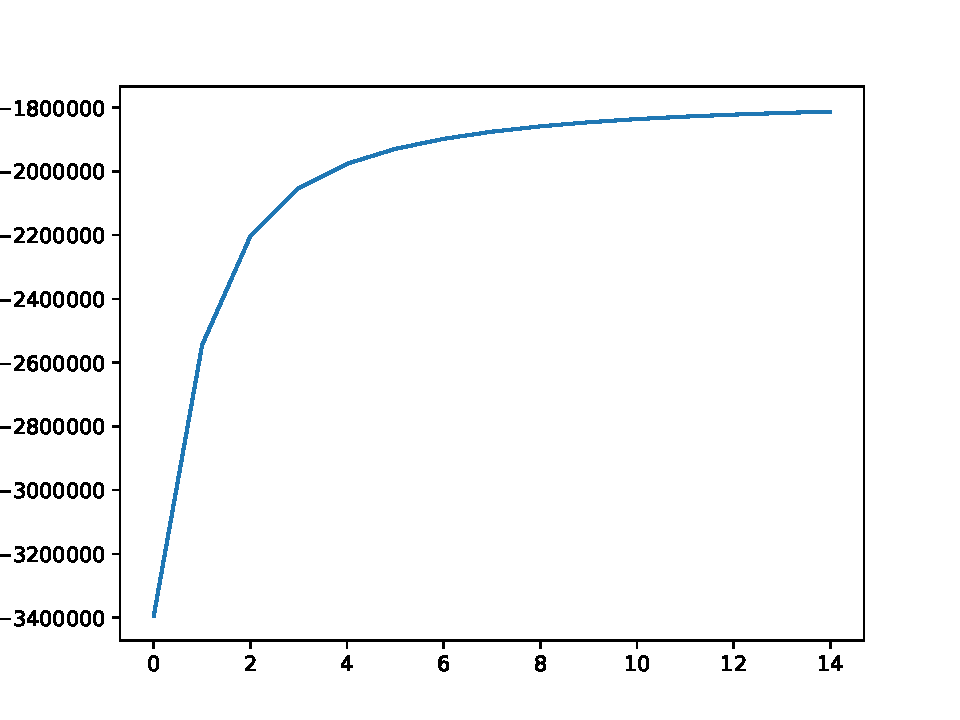
\includegraphics[width=\linewidth]{images/ELBOs.pdf}
\caption{ELBO of the IBM-VI on a 10k subset of the development set plotted per epoch}
\label{fig:VI-ELBO}
\end{figure}

\begin{figure}
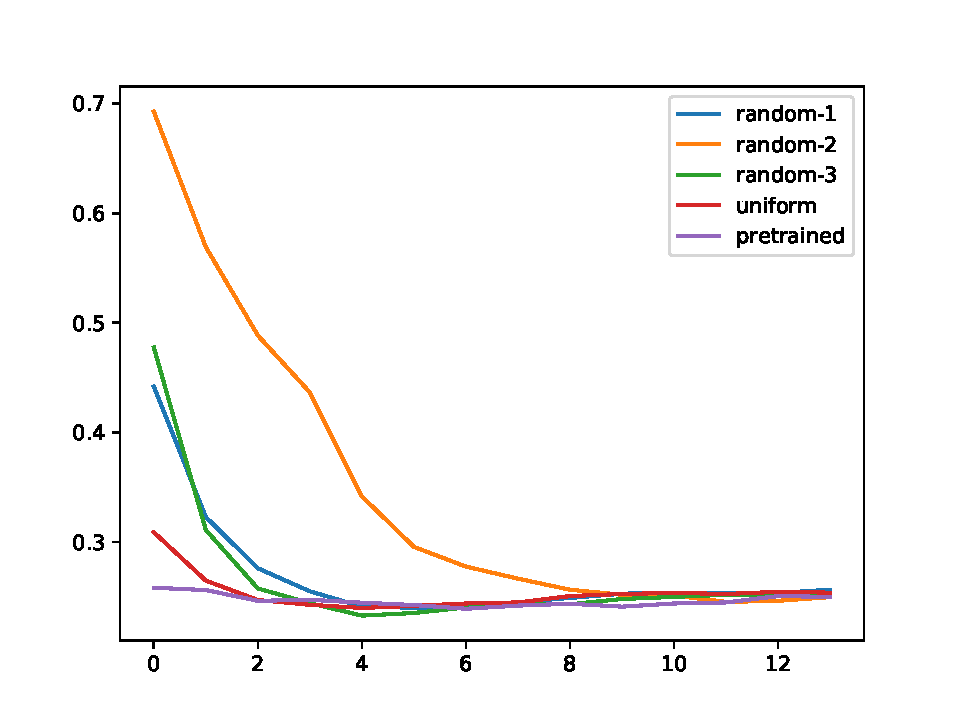
\includegraphics[width=\linewidth]{images/AERs-together.pdf}
\caption{AER on the development set for various initialisations of IBM2 plotted per epoch}
\label{fig:AERs-together}
\end{figure}

\begin{figure}
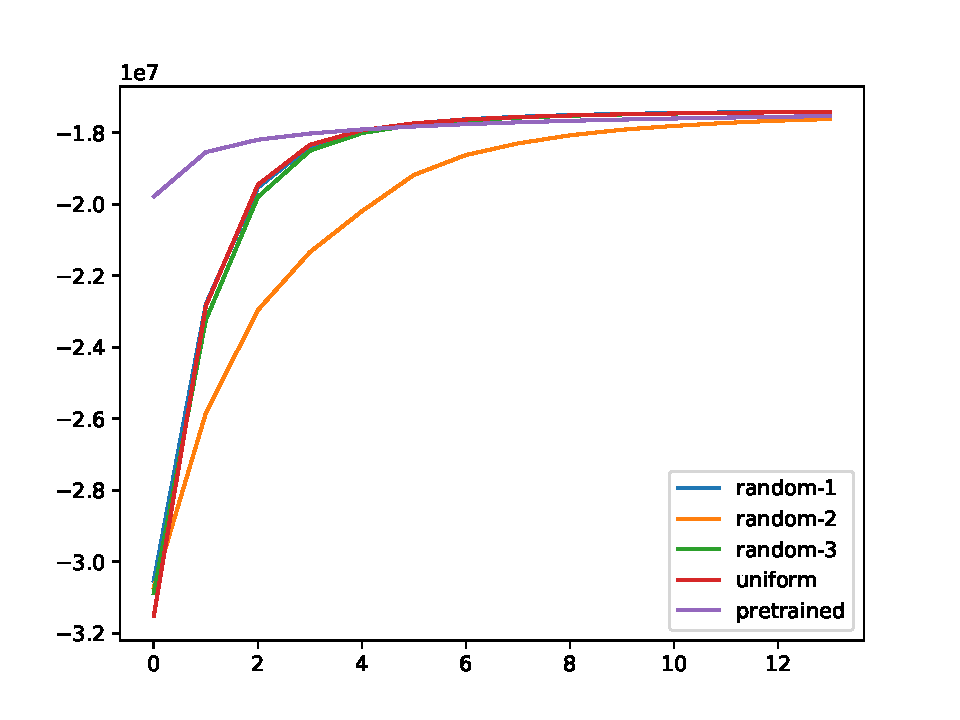
\includegraphics[width=\linewidth]{images/likelihoods.pdf}
\caption{Log-likelihood of the training set for various initialisations of IBM2 plotted per epoch}
\label{fig:AERs-together}
\end{figure}

\begin{figure}
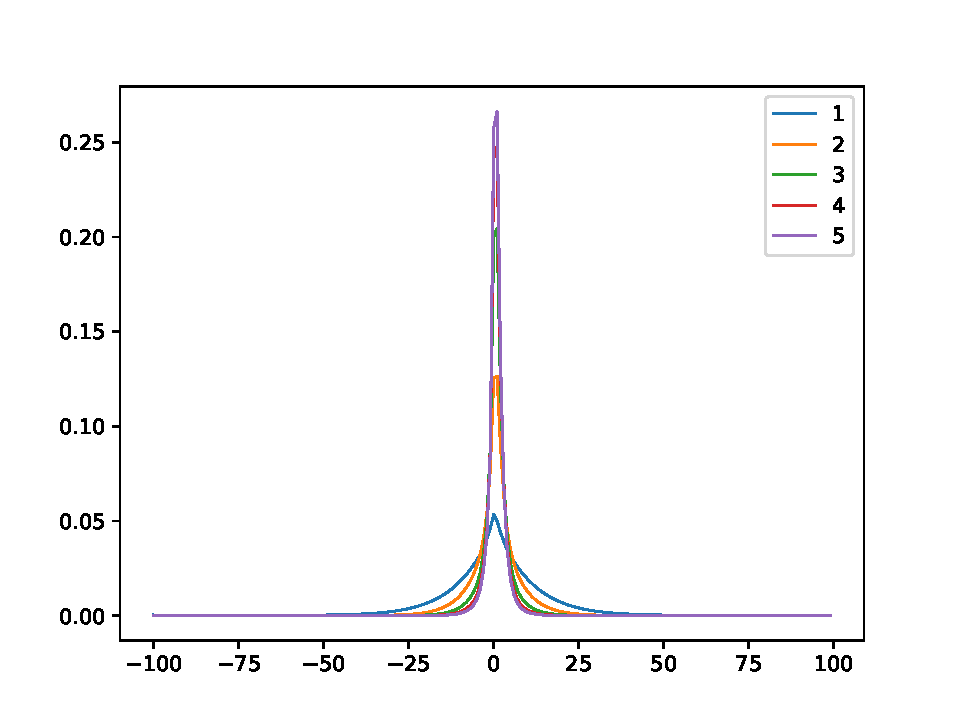
\includegraphics[width=\linewidth]{images/epoch-jump-plot.pdf}
\caption{Evolution of the jump distribution over epochs 1-5. Change becomes minimal after 5 epochs.}
\label{fig:jump-plot}
\end{figure}

\end{document}
% Data description
% Experimental setup
% Difference AER & Likelihood
% Cutoff IBM1 
% NULL words e_0

% Moore's improvements on EM.